\chapter[Metodologia]{Metodologia}

\section{Metodologia de Desenvolvimento}

Para o desenvolvimento do trabalho será adotada uma metodologia híbrida, contendo diferentes ferramentas de abordagens de desenvolvimento de software. Essa personalização tem o objetivo de otimizar ao máximo as tarefas à serem desempenhadas no contexto em que esse trabalho é desenvolvido, tendo como uma das motivações principais para realizar essa personalização o fato do trabalho ser construído sem o auxílio de outras pessoas.

Será utilizada a metodologia KanBan, com algumas personalizações, para gerenciar a execução de atividades. Os cartões utilizados neste quadro estarão representados no formato de \textit{User Story}, comumente utilizada na metodologia SCRUM, com seu conteúdo sendo composto por: uma descrição no formato da sentença \textbf{Eu como <quem>, quero <o que>, para <ação>}, as \textit{tasks} a serem desenvolvidas e o tempo limite para sua realização.

O quadro será composto por 4 diferentes colunas: A fazer, Fazendo, Aguardando Validação e Finalizados. A imagem a seguir exemplifica um fluxo de desenvolvimento utilizando-se do KanBan.

    \begin{figure}[H]
         \centering
         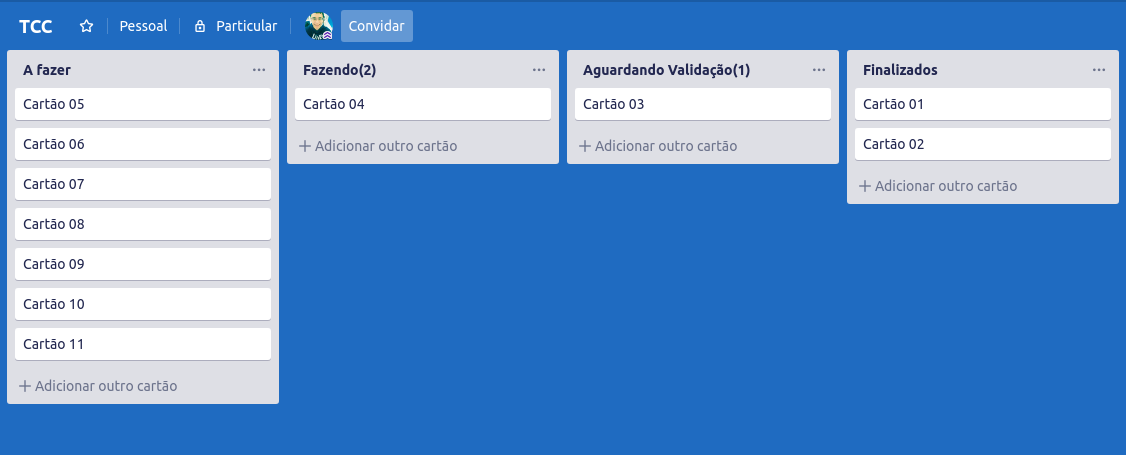
\includegraphics[scale=0.4]{figuras/capitulo_4/kanban_exemplo.png}
         \caption{KanBan formatado na ferramenta \href{https://trello.com/}{Trello}}
         \label{fig:kanban_trello_exe}
    \end{figure}

A coluna \textbf{A Fazer} funcionará como um \textit{Backlog} das funcionalidades que serão desenvolvidas ao decorrer do trabalho(possíveis bugs ou melhorias que surjam ao decorrer do projeto também serão adicionadas à essa coluna),onde os cartões posicionados acima são os considerados de maior prioridade para serem desenvolvidos. A coluna \textbf{Fazendo} será responsável por indicar a funcionalidade que está em processo de desenvolvimento. Já a \textbf{Aguardando Validação} indicará a funcionalidade que está passando por um processo de validação, como por exemplo a realização de testes com usuários reais para validar o funcionamento implementado.E a coluna \textbf{Finalizados} conterá o histórico das funcionalidades já implementadas e que foram validadas de acordo com os testes planejados.

\section{Cronograma}

